One of the first methods of additive manufacturing (AM) is stereolithography \citep{kodama1981automatic, hull1986apparatus, 3d2019our} which involves the curing of a photosensitive resin using an ultraviolet laser. The technology has evolved and AM is capable of manufacturing objects with complicated internal and external geometries, some examples are shown in Figure \ref{fig:literature_3dprint}. However, there is a need for product inspection and in particular assessing the quality of the internal structures.

\begin{figure}
  \centering
  
\includegraphics[width=0.9\textwidth]{../figures/literatureReview/literature_3dprint.png}
  \caption{Examples of additive manufactured parts: a) lattice structure, b) toy, c) chain, d) model of a facial implant, e) spanner, f) ratchet mechanism, g) toy, h) series of rotatable gears, i) lattice structure. Republished with permission of Springer New York, from \cite{gibson2010additive}; permission conveyed through Copyright
Clearance Center, Inc.}
  \label{fig:literature_3dprint}
\end{figure}

Imaging using x-rays \citep{rontgen1896on} have been used in the medical field. In x-ray computed tomography \citep{cormack1973reconstruction, hounsfield1973computerized, hounsfield1980computed}, the patient has an x-ray image taken at multiple angles. These x-ray images are used to reconstruct what was taken in 3D to make a diagnostic.

X-ray computed tomography (XCT) can be used as a non-destructive test for AM products. Various reviews on AM exist such as \cite{kruth1991material, kruth1998progress, pham1998comparison, gibson2010additive, wong2012review, ngo2018additive}. For XCT used in manufacturing, there are \cite{cantatore2011introduction, kruth2011computed, sun2012overview}. \cite{thompson2016x} reviewed the applications of XCT on AM.

In this chapter, AM is reviewed followed by XCT. The latest research for the use of XCT on AM is reviewed at the end of the chapter.

\section{Additive Manufacturing}

Loosely, AM involves solidifying material onto a moving platform so that the object is manufactured layer by layer. Typically, this is a slow and expensive method compared to destructive methods such as computer numerical control (CNC) machining for example. An advantage of AM is that the setup cost is low, in particular, destructive methods require planning and setting up various apparatus before the manufacturing stage \citep{gibson2010additive}. This makes it suitable to manufacture bespoke items which achieves the goals of AM's predecessor called rapid prototyping \citep{kruth1991material}.

Various AM technologies were invented during the advancement of AM. Because of this, there are various applications of AM, for example in medical and biomedical sciences \citep{kang20163d, kourra2018computed}, engineering \citep{cooper2015design}, food engineering \citep{godoi20163d} and art \citep{ornes2013mathematics, grossman2019bathsheba}.

\subsection{Additive Manufacturing Technologies}

The different AM technologies can be classified based on the apparatus, for example, liquid-based or powder-based, and/or on the method of manufacturing, for example, point by point or layer by layer \citep{kruth1991material}. The liquid-based AM technologies presented here are stereolithography \citep{kodama1981automatic, hull1986apparatus, 3d2019our} and fused deposition modelling \citep{crump1991fused, crump1992apparatus, stratasys2019what}. The following powder-based technologies are presented here: 3D printing \citep{sachs1990three}, selective laser sintering \citep{deckard1989method, dtm1990the, 3d2019our}, electron beam melting \citep{larsson2004arrangement, arcam2019history}, laser engineered net shaping \citep{atwood1998laser}. Illustrations of these technologies are shown in Figure \ref{fig:literature_technologies}.

\begin{figure}
  \centering
  \centerline{
    \begin{subfigure}[b]{0.59\textwidth}
      
\includegraphics[width=\textwidth]{../figures/literatureReview/literature_technologies_stl.png}
      \caption{Stereolithography}
    \end{subfigure}
    \begin{subfigure}[b]{0.39\textwidth}
      
\includegraphics[width=\textwidth]{../figures/literatureReview/literature_technologies_fdm.png}
      \caption{Fused deposition modelling}
    \end{subfigure}
  }
  \centerline{
    \begin{subfigure}[b]{0.7\textwidth}
      
\includegraphics[width=\textwidth]{../figures/literatureReview/literature_technologies_3dp.png}
      \caption{3D printing}
    \end{subfigure}
  }
  \centerline{
    \begin{subfigure}[b]{0.7\textwidth}
      
\includegraphics[width=\textwidth]{../figures/literatureReview/literature_technologies_laser.png}
      \caption{Selective laser sintering}
    \end{subfigure}
  }
  \caption{Diagrams of various AM technologies. Reprinted from \cite{wang20173d}\textsuperscript{\textcopyright}, with permission from Elsevier.}
  \label{fig:literature_technologies}
\end{figure}

Stereolithography is a liquid-based AM technology. It consists of a container containing a liquid photo-hardening monomer or polymer as well as a piston and platform which holds and moves the manufactured product up and down. A laser with a specific wavelength, typically \SIrange{300}{400}{\nano\metre} \citep{kodama1981automatic}, is emitted onto a point of the surface of the liquid and solidifies. The laser is controlled by a computer to solidify specific parts of the liquid surface. The platform is lowered and the cycle repeats, manufacturing the object layer by layer. Laser absorption happens a few tenths of a millimetre which corresponds to the thickness of each layer \citep{kruth1991material, pham1998comparison}.

Fused deposition modelling is another liquid-based AM technology. A jetting head, or nozzle, deposit the molten material onto a platform or on top of the previous layer. The material is usually plastic in the form of a thin filament. It is heated to just above its melting points, typically \SI{1}{\degreeCelsius} \citep{crump1992apparatus}, so that it cools down within \SI{0.1}{\second} \citep{kruth1991material}. The platform moves, and controlled by a computer, in the $xy$ plane, or left to right and front to back, to produce a layer. The jetting head can move in the $z$-axis, or up and down, to manufacture the next layer. In the original patent by \cite{crump1992apparatus}, the thickness can be as thin as 0.000\,1 inches (\SI{0.003}{\milli\metre}).

3D printing is a powder-based AM technology. A jetting head deposits a binding agent in droplets onto a bed of powder of ceramic, metal or polymer. The binding agent is cured via evaporation or heating which glues the powder particles together. The jetting head can move in the $xy$-plane and the object is manufactured layer by layer by moving the platform in the $z$-axis and renewing the powder using a roller. The binding agent must have a low viscosity so it can be deposited and may also be charged so that it can be deflected using an electric field for precise deposition \citep{sachs1990three}. The thickness of each layer is determined by the size of the droplets of the binding agent, which can be as small as \SI{15}{\micro\metre} in diameter \citep{sachs1990three}. \cite{sachs1990three} reported a tolerance of 0.001 inches (\SI{0.03}{\milli\metre}).

Selective laser sintering, electron beam melting and laser engineered net shaping are powder-based AM technology. Selective laser sintering is similar to 3D printing, but instead, a laser is used to sinter or fuse the powder particles in a chamber heated just below the melting point of the material \citep{wong2012review}. Various materials such as metals and plastics can be used \citep{wong2012review}. Electron beam melting is similar, but instead of a laser, an electron beam is used. This is done in a high vacuum chamber to avoid oxidation \citep{wong2012review}. In laser engineered net shaping, a powder bed is not used; the powder is deposited on the desired location and then melted using a laser, as shown in Figure \ref{fig:literature_lens}. This is a popular method to manufacture metal objects \citep{gibson2010additive}.

\begin{figure}
  \centering
  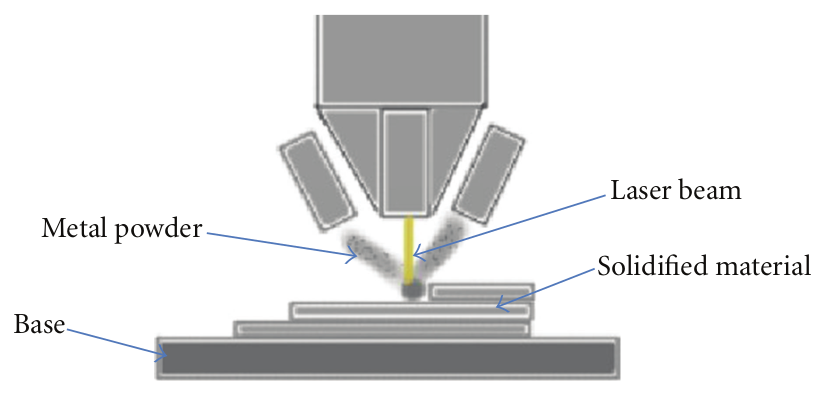
\includegraphics[width=0.7\textwidth]{../figures/literatureReview/literature_lens.png}
  \caption{Laser engineered net shaping. Reprinted from \citep{wong2012review} under the CC BY 3.0 license.}
  \label{fig:literature_lens}
\end{figure}

There are many more AM technologies but they can be found in numerous review literature. A comparison of the mentioned AM technologies available at the time was done by \cite{pham1998comparison, kim2008benchmark}. Factors such as material cost, mechanical properties and the resolution of the manufacturing were considered. There are also safety aspects to assess, for example, powder in powder-based methods can escape into the environment and the liquid used in stereolithography is toxic, sticky and has spilling risk \citep{kim2008benchmark}. This makes fused deposition modelling a popular choice and can be used in an office environment \citep{ngo2018additive}.

The strength of the manufactured object varies from geometry to geometry but also from direction to direction. Because the manufactured object is made layer by layer, the strength varies if the load was applied in the building direction (vertical) or the scanning direction (horizontal) \citep{kim2008benchmark}. Experimental results have shown that fused deposition modelling has superior strength in the scanning direction but weak in the building direction \citep{kim2008benchmark}.

The strongest manufacturing methods were found to be powder-based methods and stereolithography, however, they are slow and material costs are high \citep{kim2008benchmark}. Fused deposition modelling has low costs and high speeds but suffers from weak mechanical properties \citep{ngo2018additive}.

The materials available for each AM technology varies. The materials used in stereolithography is limited because of the use of liquids with photo-hardening properties \citep{ngo2018additive}. Fused deposition modelling is limited to plastics \citep{ngo2018additive}. Selective laser sintering and laser engineered net shaping can manufacture objects using metals such as aluminium alloys, steel, titanium and titanium alloys \citep{herzog2016additive}.

\subsection{Pre/Post Processing}

The blueprint of the object to be manufactured is called a computer-aided design (CAD) model. For it to be processed by an AM apparatus, the CAD model is converted to an STL file \citep{3d1989sterolithography, 3d2019what} which represent surfaces by a series of triangles, an example is shown in Figure \ref{fig:literature_stl}. STL stands for stereolithography but could also be called standard tessellation language \citep{wong2012review}. Some accuracy is lost here as the surface of the CAD model is represented approximately by triangles \citep{gibson2010additive}. The STL file is then sliced into layers \citep{jamieson1995direct, vatani2009enhanced} so that the AM apparatus knows what to build for each layer.

\begin{figure}
  \centering
  
\includegraphics[width=0.9\textwidth]{../figures/literatureReview/literature_stl.png}
  \caption{An example of a CAD model (left) converted to a STL file (right). Republished with permission of Springer New York, from \cite{gibson2010additive}; permission conveyed through Copyright
Clearance Center, Inc.}
  \label{fig:literature_stl}
\end{figure}

When the AM object is manufactured, post-processing techniques can be done at this stage. For example, sanding may be done to smooth the surfaces \citep{gibson2010additive}. The manufactured object may be inspected for pores or defects by comparing the x-ray projection of the object with the CAD model \citep{lee2015compliance, villarraga2015assessing, kim2016inspection}.

As with any apparatus, regular maintenance is required \citep{bell2014maintaining}.

\subsection{Defects and Quality Control}

There are various discontinuities in AM. In FDM, a staircase effect on the surface of the product arises from poor slicing methods of the CAD model \citep{weeren1995quality}. Internal voids can be formed due to insufficient material flow \citep{weeren1995quality}. Other factors which can cause defects include misalignment of the platform or nozzle, depletion of material and lack of adhesion due to low temperatures \citep{gunaydin2018common}.

There are also problems in the manufacturing of metal parts \citep{everton2016review}, for example, gas can become trapped during the manufacturing process forming gas pores in the manufactured object \citep{thijs2010study, tammas2015xct}. These gas pores can be \SIrange{5}{20}{\micro\metre} in diameter \citep{everton2016review}.

Layers may not fuse and form elongated pores. This can be fixed by increasing the energy of the beam but increasing it too much will cause evaporation of the AM part \citep{mumtaz2008high}. These pores can be \SIrange{50}{500}{\micro\metre} in size \citep{everton2016review} and can be observed using a scanning electron microscope as shown in Figure \ref{fig:literature_pores}.

Low wetting ability of the melt pool can cause balling which is where the sintered powder has poor contact on the existing layer causing spherical particles to form on the surface of the AM part \citep{li2012balling, gu2009balling}. The spherical particles can vary in size of \SIrange{10}{500}{\micro\metre} \citep{li2012balling}. The balling effect can be reduced by ensuring low oxygen content in the environment \citep{niu1999instability} and using higher energy beams \citep{gu2009balling}. Some examples are shown in Figure \ref{fig:literature_balling} using an electron scanning microscope.

Cracks can form due to extreme temperature changes and gradients \citep{mercelis2006residual, zaeh2010investigations}.

\begin{figure}
  \centering
  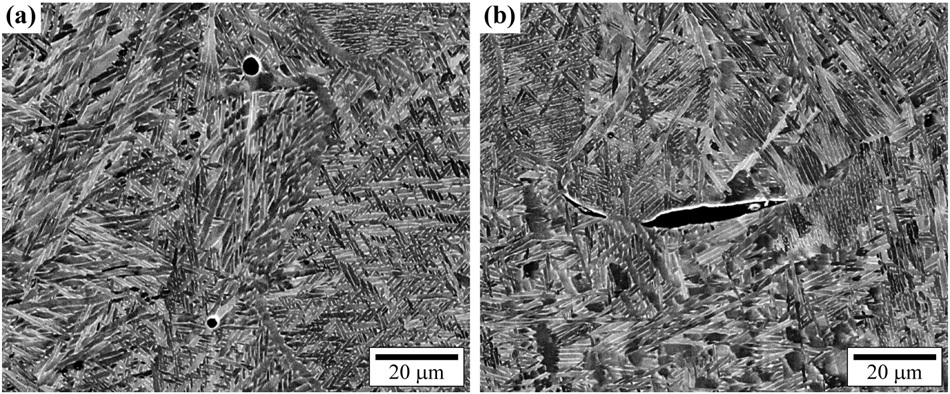
\includegraphics[width=0.99\textwidth]{../figures/literatureReview/literature_pores.png}
  \caption{A scanning electron microscope image of a) pores and b) elongated pores from an electron beam melting manufactured object. Reprinted from \cite{tammas2015xct} under the CC BY 4.0 license.}
  \label{fig:literature_pores}
\end{figure}

\begin{figure}
  \centering
  
\includegraphics[width=0.7\textwidth]{../figures/literatureReview/literature_balling.png}
  \caption{A scanning electron microscope image of balling on a selective laser melting manufactured object. Reprinted by permission from Springer Nature: \cite{li2012balling}\textsuperscript{\textcopyright}.}
  \label{fig:literature_balling}
\end{figure}

The manufacturing process can be monitored, this is called online or in-situ process monitoring \citep{everton2016review}. The idea is that problems during the manufacturing process are found as soon as possible before the final product is spoiled \citep{cerniglia2015inspection}. Various methods are used for in-situ process monitoring, for example, a high-speed camera can be installed to capture the various wavelengths in the electromagnetic spectrum emitted by the melt pool \citep{berumen2010quality, craeghs2011online, lott2011design}. Various discontinuities and errors can be detected \citep{clijsters2014in} and be used to give feedback to the AM apparatus \citep{herzog2013method}. Other methods include measuring the surface using a laser \citep{cerniglia2015inspection} and using an infrared camera to measure the temperature of the melt pool \citep{rodriguez2012integration}. 

\section{X-ray Computed Tomography}

XCT started its use in the medical field but the advancement of the technology saw its use in manufacturing and metrology, the science of measurement. Applications of XCT include the examination of acetabular hip prosthesis cups \citep{kourra2018computed}, skeletons \citep{appleby2014scoliosis}, batteries \citep{taiwo2017investigating} and materials \citep{zhang2016x, wang2017x}. XCT can be used to reverse engineer existing products and improvements can be fabricated using AM, for example, it was used for improving existing hollow engine valves \citep{cooper2015design}. However, the use of XCT in metrology is not yet firmly established compared to other methods of measurement \citep{thompson2016x}. This is because there are a lot of inconsistencies in the setup of XCT apparatuses and on controlling the sources of error.

\subsection{Concepts from the Medical Field}

The setup of XCT \citep{cormack1973reconstruction, hounsfield1973computerized, hounsfield1980computed} in the medical field involves the patient laying on a flatbed. An x-ray source and x-ray detector pair rotate around and translate along the patient to get readings of the x-rays after attenuating through the patient via different paths. X-ray beams were pencil beams in the early versions of XCT \citep{michael2001x}. To reduce scanning times, fan-shaped beams and arrays of detectors were used and they can move in a spiral fashion along and around the patient \citep{cierniak2011x}. These multiple x-ray readings can be used to reconstruct a representation of the patient in 3D \citep{zeng2010medical}. This is illustrated in Figure \ref{fig:literature_medicalct}.

\begin{figure}
  \centering
  
\includegraphics[width=0.99\textwidth]{../figures/literatureReview/literature_medicalct.png}
  \caption{In medical XCT, a fan-shaped x-ray beam is emitted and attenuate through the patient and detected by a detector. The x-ray source and detector rotate around and translate along the patient. By collecting readings at different angles, the image of the patient can be reconstructed. Reprinted from \cite{michael2001x}. \textcopyright\ IOP Publishing. Reproduced with permission. All rights reserved.}
  \label{fig:literature_medicalct}
\end{figure}

The patient cannot be exposed to too much radiation, therefore the x-rays used are of low power which can cause noisy readings from the detector. The sources of noise are from the behaviour of the x-rays and the electronics in the detector \citep{yang2010noise}. In this realm of low signal to noise ratio, the noise has a compound Poisson element to it \citep{whiting2002signal, whiting2006properties}. Many reconstruction algorithms have been proposed to consider the compound Poisson noise \citep{elbakri2002statistical, elbakri2003efficient, elbakri2003statistical, lasio2007statistical, xie2008x}.

\subsection{Acquisition Process in Manufacturing}

In manufacturing and metrology, high power x-rays can be used in XCT because there is no consequence of the manufactured object absorbing the radiation. As a result, the XCT setup is different. The object is held by foam on a turntable and placed between an x-ray source and an x-ray detector. X-ray projections are taken while the object rotates. Typically the x-ray is a cone-beam \citep{kruth2011computed}. This is illustrated in Figure \ref{fig:literature_xct}.

\begin{figure}
  \centering
  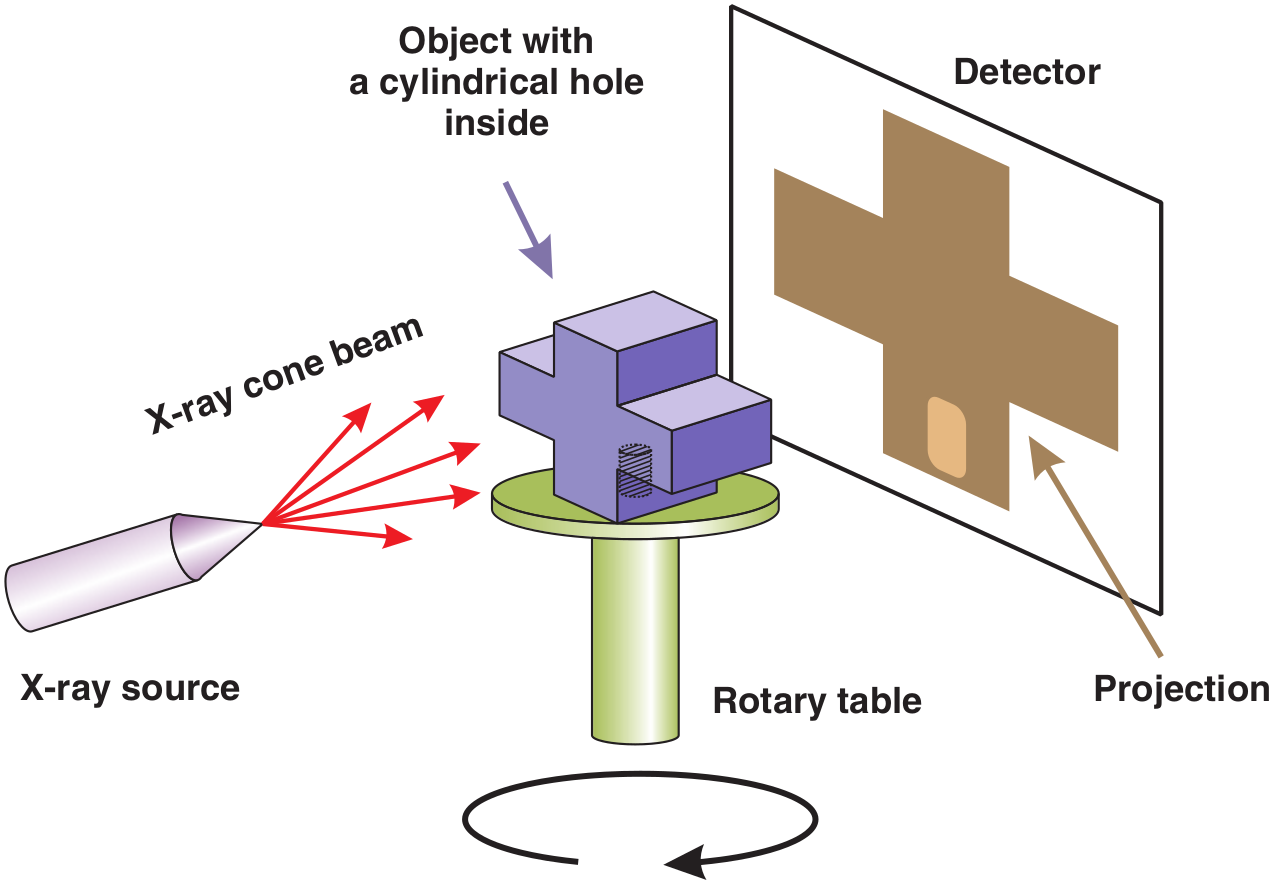
\includegraphics[width=0.75\textwidth]{../figures/literatureReview/literature_xct.png}
  \caption{The setup of XCT used in metrology. Reprinted from \cite{warnett2016towards} under the CC BY 3.0 license.}
  \label{fig:literature_xct}
\end{figure}

The acquisition process consists of the production of x-rays, x-rays attenuating the object, the detection of x-rays and the reconstruction process.

X-rays \citep{rontgen1896on} are produced in an x-ray tube, a diagram shown in Figure \ref{fig:literature_tube}. It consists of a vacuum tube containing a cathode and an anode. Electrons are fired from the cathode to the anode due to an electric potential. The cathode is usually tungsten and the anode contains a small amount of tungsten, molybdenum or copper \citep{sun2012overview}.

\begin{figure}
  \centering
  
\includegraphics[width=0.8\textwidth]{../figures/literatureReview/literature_tube.png}
  \caption{An x-ray tube. Reprinted from \cite{michael2001x}. \textcopyright\ IOP Publishing. Reproduced with permission. All rights reserved.}
  \label{fig:literature_tube}
\end{figure}

The electrons can interact with the anode in many ways. The electrons can be deflected or decelerated due to the electric field from the nucleus of the target anode material. The energy lost by the electrons is emitted as bremsstrahlung radiation. The energy of the radiation depends on the potential difference in the x-ray tube, as this determines the energy of the fired electrons, and also the proton number of the anode target because this affects the electric field produced by the nucleus in the anode target \citep{sun2012overview}. Another interaction is when the electrons may collide with the nucleus in the anode target, exciting an inner shell electron and ionizing it. This produces a vacancy in the electron shell and emits a photon when the excited electron drops down back to the ground state. This is known as characteristic radiation and the energy emitted is discrete and depends on the material in the anode target \citep{sun2012overview}.

The efficiency of an x-ray tube is poor. Over 99\% of the energy from electrons is converted to heat, the rest to x-rays \citep{kruth2011computed}.

Photons, making up the radiation, are emitted from the x-ray tube which can be modelled as a Poisson process \citep{whiting2006properties, cierniak2011x}. The rate of x-ray emission depends on the current, that is the rate of charge between the cathode and anode. Sources of energy of each photon come from bremsstrahlung radiation and characteristic radiation, making the distribution of x-ray photons energy a mix of continuous and discrete energies \citep{sun2012overview}. An example is shown in Figure \ref{fig:literature_spectrum}.

\begin{figure}
  \centering
  
\includegraphics[width=0.65\textwidth]{../figures/literatureReview/literature_spectrum.png}
  \caption{An example of the distribution of energies a photon can have emitted from an x-ray tube. Bremsstrahlung and characteristic radiation contribute to the continuous and discrete components of the distribution. Reprinted from \cite{michael2001x}. \textcopyright\ IOP Publishing. Reproduced with permission. All rights reserved.}
  \label{fig:literature_spectrum}
\end{figure}

The scanned object is exposed to x-ray photons which undergo attenuation when interacting with the object in several ways \citep{cantatore2011introduction}. The object can absorb the photons via the photoelectric effect. In the photoelectric effect, a photon transfer all of its energy to a bounded electron and ejects it from the atom in the object \citep{millikan1916direct}. Photons can be scattered by the object by colliding inelastically with and transfers its energy to an electron. This process is known as Compton scattering \citep{compton1923quantum}. The photoelectric effect and Compton scattering cause several photons to be undetectable. If some of the photons avoid these processes, they are detected and their energy is left unaffected.

Beer's law simplifies these quantum mechanistic process. Suppose the x-ray beam with a rate of emission $I_0$ is mono-energetic and travels in a straight line in the $x$-axis. Let $\mu(x)$ be the attenuation coefficient of the object and the x-ray beam has a rate of emission $I$ after attenuation. A differential equation can be set up to model the decay of photons as it attenuates through the object such that
\begin{equation}
\dfrac{\diff I}{\diff x} = -I\mu(x)
\end{equation}
which can be solved
\begin{equation}
I = I_0\exp\left[\int_{x \in \text{path of photon}}-\mu(x)\diff x\right] \ .
\label{eq:beerLaw}
\end{equation}
However, the photoelectric effect and Compton scattering, thus the attenuation coefficient as well, depends on the energy of the photons \citep{elbakri2002statistical}. Therefore $\mu(x,E)$ should be made dependent on the energy of the photons \citep{cantatore2011introduction} and can cause some inaccuracies in Beer's law. In general low energy photons are more likely to be absorbed and scattered than high energy photons, which increases the average energy of the detected photons \citep{sun2012overview}. This is called beam hardening.

After attenuation, the x-ray photons are detected by the x-ray detector. The detectors used in XCT are typically flatbed scanners made up of a scintillator material \citep{curran1953luminescence, greskovich1997ceramic} and photodiodes. The x-ray photons interact with the scintillator material and produce visible light pluses \citep{rossner1993conversion}. These pulses are detected by photodiodes and converted into an electrical signal \citep{nikl2006scintillation, ren2018tutorial}. The electrical signal can be a quantum counter, counting the number of photons detected, or an energy integrating detector, adding up all of the energies of each detected photon \citep{nikl2006scintillation, whiting2006properties, kruth2011computed, ren2018tutorial}. The electrical signals are subject to sampling and quantisation to store these signals as an image \citep{cierniak2011x}. This image is known as a projection.

Not all of the visible light pulses are detected by the photodiodes, thus not all the x-ray photons are detected. The ratio between the number of x-ray photons detected by the detector and the number of x-ray photons arriving at the detector is called the quantum efficiency \citep{cierniak2011x, ren2018tutorial}. This makes the detection a two-stage process, converting the x-ray photons into visible light which are then detected \citep{cierniak2011x}. There exist equipment which detects x-ray directly such as a xenon gas ionisation detector \citep{fuchs2000direct} but this is unrivalled by solid-state CT systems, such as scintillator-photodiodes detectors, which have a high quantum efficiency of about 98\% to 99.5\% \citep{hsieh2000investigation}.

Once projections of the object have been acquired at multiple angles, the reconstruction process can start. The objective of reconstruction is to estimate the attenuation coefficient of the object at each point in space $\mu(x,y,z)$ using the x-ray projections. This is done using the fact that the projections are based on the line integral of the attenuation coefficient along the path of photons. This problem was formed by \cite{radon1986on} as the `determination of functions from their integral values along certain manifolds'.

A number of reconstruction algorithms in XCT have been developed \citep{smith1990cone} such as the filtered back-projection \citep{brooks1976principles} and the FDK algorithm \citep{feldkamp1984practical}. Once the reconstruction has been done, the shape or surface can be extracted by the use of thresholding \citep{kruth2011computed}. There are many software packages available for the reconstruction stage of XCT \citep{reinhart2008industrial, sun2012overview}.

\subsection{Metrology in Practice}

XCT can be used to measuring lengths and distances, making it useful for measuring the dimensions of AM objects internally and externally. \emph{Nikon} offer products and services for XCT including features such as direct comparison to the CAD model \citep{nikon2015microfocus, nikon2018mct225} and automated production line inspection \citep{nikon2015inline, nikon2018automated}.

As with a lot of measurement apparatus, calibration is required. In XCT, the scale of each voxel in the reconstruction can be obtained by using XCT on an object with pre-determined lengths, these are known as reference standards \citep{bartscher2007enhancement} but can have similar names. Reference standards can vary in geometry such as a sphere on a cylinder \citep{lifton2013application}, two spheres on a cylinder \citep{sun2016reference}, a cube with cut-outs \citep{kiekens2011test}, a hollow cylinder, a step-cylinder and a ball-bar \citep{bartscher2007enhancement}; the latter three are shown in Figure \ref{fig:literature_referenceStandards}.

\begin{figure}
  \centering
  \centerline{
    \begin{subfigure}[b]{0.49\textwidth}
      
\includegraphics[width=\textwidth]{../figures/literatureReview/literature_test1.png}
      \caption{Hollow cylinder}
    \end{subfigure}
    \begin{subfigure}[b]{0.49\textwidth}
      
\includegraphics[width=\textwidth]{../figures/literatureReview/literature_test2.png}
      \caption{Step-cylinder}
    \end{subfigure}
  }
  \begin{subfigure}[b]{0.6\textwidth}
    
\includegraphics[width=\textwidth]{../figures/literatureReview/literature_test3.png}
    \caption{Ball-bar}
  \end{subfigure}
  \caption{Various reference standards: a) aluminium hollow cylinder, outer diameters \SI{30}{\milli\metre} and \SI{20}{\milli\metre}, b) aluminium step-cylinder with diameter \SI{300}{\milli\metre}, c) ceramic balls of diameter \SI{30}{\milli\metre} on a carbon fibre rod, the balls are separated by \SI{100}{\milli\metre}. Reprinted from \cite{bartscher2007enhancement}\textsuperscript{\textcopyright} with permission from Elsevier.}
  \label{fig:literature_referenceStandards}
\end{figure}

There are many variables in XCT and a lot of them have to be controlled, for example, XCT should be done in room temperature to avoid any thermal variation \citep{bryan1990international}, however, this can be hard to do when the x-ray tube is a heat source \citep{kruth2011computed}.

The potential difference and current of the x-ray tube can be adjusted to control the contrast and brightness of the x-ray projection. The exposure time is also a factor. These settings should be set high enough to avoid beam extinction but low enough that there is a contrast where less material is present \citep{kruth2011computed}.

The magnification can be modified by altering the distances between the x-ray tube, the object and the x-ray detector. Increasing the magnification increases the image resolution but can cause blurry images, this is the result of using an x-ray source with a finite spot size as shown in Figure \ref{fig:literature_magnification} \citep{kruth2011computed}. Larger spot sizes cause more blurry results, this is known as the penumbra effect \citep{kueh2016modelling}. However, spot sizes too small can produce concentrated heat \citep{welkenhuyzen2009industrial} and can damage the x-ray tube.

\begin{figure}
  \centering
  
\includegraphics[width=0.7\textwidth]{../figures/literatureReview/literature_magnification.png}
  \caption{The magnification can be adjusted by adjusting the distances between the x-ray source, the object and the x-ray detector. Because of a finite x-ray spot size, blurry effects are produced using a magnification too large. Reprinted from \cite{kruth2011computed}\textsuperscript{\textcopyright} with permission from Elsevier.}
  \label{fig:literature_magnification}
\end{figure}

There is also the question on how to orient the object on the turntable \citep{corcoran2016observations} as well as how many angles to use \citep{kruth2011computed}. More angles produce a more accurate reconstruction but require more acquisition time. Figure \ref{fig:literature_angles} shows an example of a reconstruction using various numbers of angles.

\begin{figure}
  \centering
  
\includegraphics[width=0.7\textwidth]{../figures/literatureReview/literature_angles.png}
  \caption{A reconstruction when scanning three aligned balls using a different number angular projections. Reprinted from \cite{kruth2011computed}\textsuperscript{\textcopyright} with permission from Elsevier.}
  \label{fig:literature_angles}
\end{figure}

All of the parameters of XCT discussed can be determined before the XCT process by use of simulations \citep{reisinger2011simulation, reiter2011simulation}, however, there may be inconsistencies. For example, even though the target material of the anode and power is specified, the energy spectrum can still vary \citep{stumbo2004direct}.

Problems can occur in the detector, for example, pixels in the acquired projection can be defective or dead \citep{brettschneider2014spatial} and the panel structure of the detector can be observed \citep{yang2009evaluation}. Another problem is that there exist spatially correlated noise within a projection which can be detected experimentally \citep{sun2016characterisation} as well as a correlation between acquisitions, known as image lag \citep{yang2009evaluation}. Precautions can be taken to reduce the impact from image lag such as waiting for 20 minutes between acquisitions \citep{yang2010noise}.

Errors due to beam hardening can occur. Low energy photons are more likely to be absorbed or scattered, which causes a few millimetres of the surface of the object to absorb or scatter more photons than the interior. This can cause artefacts \citep{sun2016applications} such as flat surfaces to be barrelled and edges rounded off \citep{kruth2011computed}. Beam hardening can be tackled by eliminating the low energy photons by placing a filter, a thin metal plate, in front of the x-ray tube \citep{welkenhuyzen2009industrial}, for example, copper. Figure \ref{fig:literature_hardening} shows an example of reconstruction with and without a filter. Without the filter, the outer perimeter appears less dense than it should be.  A filter reduces the rate of photon emission but this can be compensated by increasing the exposure time \citep{kruth2011computed}. Early reconstruction algorithms ignored beam hardening but modern methods can take beam hardening into account \citep{elbakri2001statistical, sun2016applications}.

\begin{figure}
  \centering
    \begin{subfigure}[b]{0.4\textwidth}
      
\includegraphics[width=\textwidth]{../figures/literatureReview/literature_hardening_noFilter.png}
      \caption{No filter}
    \end{subfigure}
    \begin{subfigure}[b]{0.4\textwidth}
      
\includegraphics[width=\textwidth]{../figures/literatureReview/literature_hardening_filter.png}
      \caption{Al/Cu filter}
    \end{subfigure}
  \caption{A reconstruction of a hollow cylinder, outer diameter \SI{6.0}{\milli\metre} and inner diameter \SI{0.6}{\milli\metre}. In a), no filter was used. In b) a filter was placed in front of the x-ray tube. Reprinted from \citep{kruth2011computed}\textsuperscript{\textcopyright} with permission from Elsevier}
  \label{fig:literature_hardening}
\end{figure}

The most common reconstruction method is the FDK \citep{feldkamp1984practical} algorithm because it caters for cone beams. However, it assumes a circular trajectory from the source which can cause artefacts if the trajectory is not circular \citep{sun2016applications}.

\subsection{Latest Research}

The most common use of XCT in AM is the investigation of pores in the manufactured object \citep{thompson2016x}. Pores can be classified as defects if the pores are larger than some volume threshold. This threshold controls the probability of the detection of defects \citep{gandossi2010probability, amrhein2014characterization}.

The porosity is defined by dividing the volume of all of the pores by the volume of solid material \citep{taud2005porosity}. This can be used to quantified the material's strength and can be measured accurately using Archimedes' method \citep{spierings2011comparison}. Studies have been done to link porosity to stress concentration \citep{leuders2015fatigue, siddique2015computed, carlton2016damage} and it was found the location of the pores is a good predictor of fatigue strength \citep{leuders2015fatigue}. XCT can be used to measure porosity and has an advantage over Archimedes' method because the location of the pores can be visualised in XCT. An example of visualising pores is shown in Figure \ref{fig:literature_pores3D} and the pores can be compared to the CAD model \citep{lee2015compliance, villarraga2015assessing, kim2016inspection}. In addition to pores, any surface deviation can be measured by aligning the reconstruction with the CAD model and measuring any discrepancies \citep{lee2015compliance, villarraga2015assessing, kim2016inspection}, an example is shown in Figure \ref{fig:literature_warnett}.

\begin{figure}
  \centering
      \begin{subfigure}[b]{0.49\textwidth}
      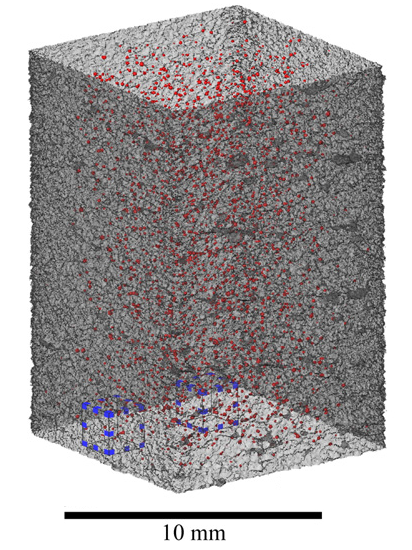
\includegraphics[width=\textwidth]{../figures/literatureReview/literature_pores3D1.png}
      \caption{Reconstruction}
    \end{subfigure}
    \begin{subfigure}[b]{0.49\textwidth}
      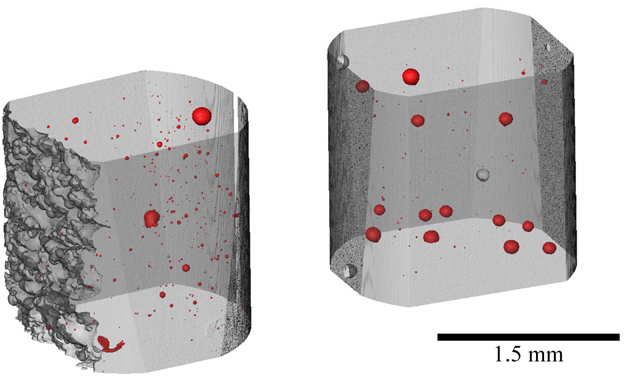
\includegraphics[width=\textwidth]{../figures/literatureReview/literature_pores3D2.png}
      \caption{Sample from the reconstruction}
    \end{subfigure}
    \caption{The reconstruction can show pores in the manufactured object. b) shows the reconstructed samples from the blue cubes in a). Reprinted from \cite{tammas2015xct} under the CC BY 4.0 license.}
    \label{fig:literature_pores3D}
\end{figure}

\begin{figure}
  \centering
      \begin{subfigure}[b]{0.49\textwidth}
      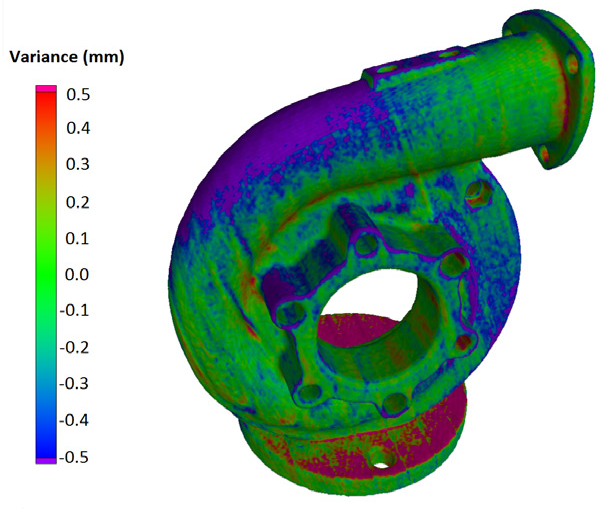
\includegraphics[width=\textwidth]{../figures/literatureReview/literature_warnett1.png}
      \caption{External}
    \end{subfigure}
    \begin{subfigure}[b]{0.49\textwidth}
      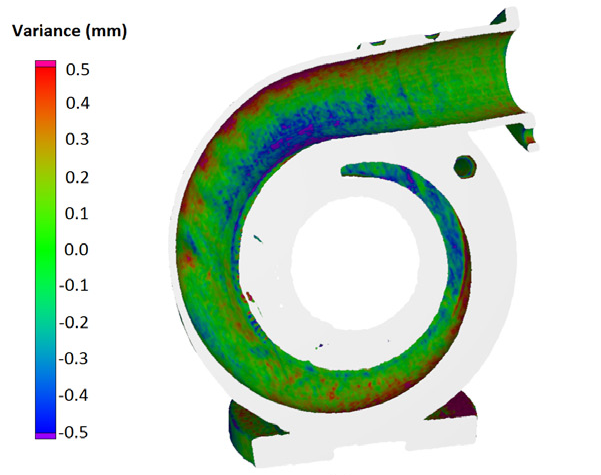
\includegraphics[width=\textwidth]{../figures/literatureReview/literature_warnett2.png}
      \caption{Internal}
    \end{subfigure}
    \caption{The reconstruction was aligned and compared to the CAD model. The surface heat map shows the surface deviation (or `variance' in the literature) externally (a) and internally (b). Reprinted from \cite{warnett2016towards} under the CC BY 3.0 license.}
    \label{fig:literature_warnett}
\end{figure}

One of the disadvantages of XCT is that it is a slow process. XCT is not an instantaneous process so progress bars are usually featured in XCT marketing such as \cite{nikon2015inline}'s inline quality control. The reconstruction can take between 5 minutes to several hours \citep{warnett2016towards}. More angular projections would take more time but will improve the accuracy of the reconstruction \citep{kruth2011computed}. \cite{warnett2016towards} improved the speed of XCT by sacrificing the accuracy of the reconstruction. This was done by placing the object on a conveyor belt surrounded by multiple x-ray source and detector pairs as shown in Figure \ref{fig:literature_conveyor}. Fewer angular projections were taken but they can be obtained in one go, speeding up the process.

\begin{figure}
  \centering
  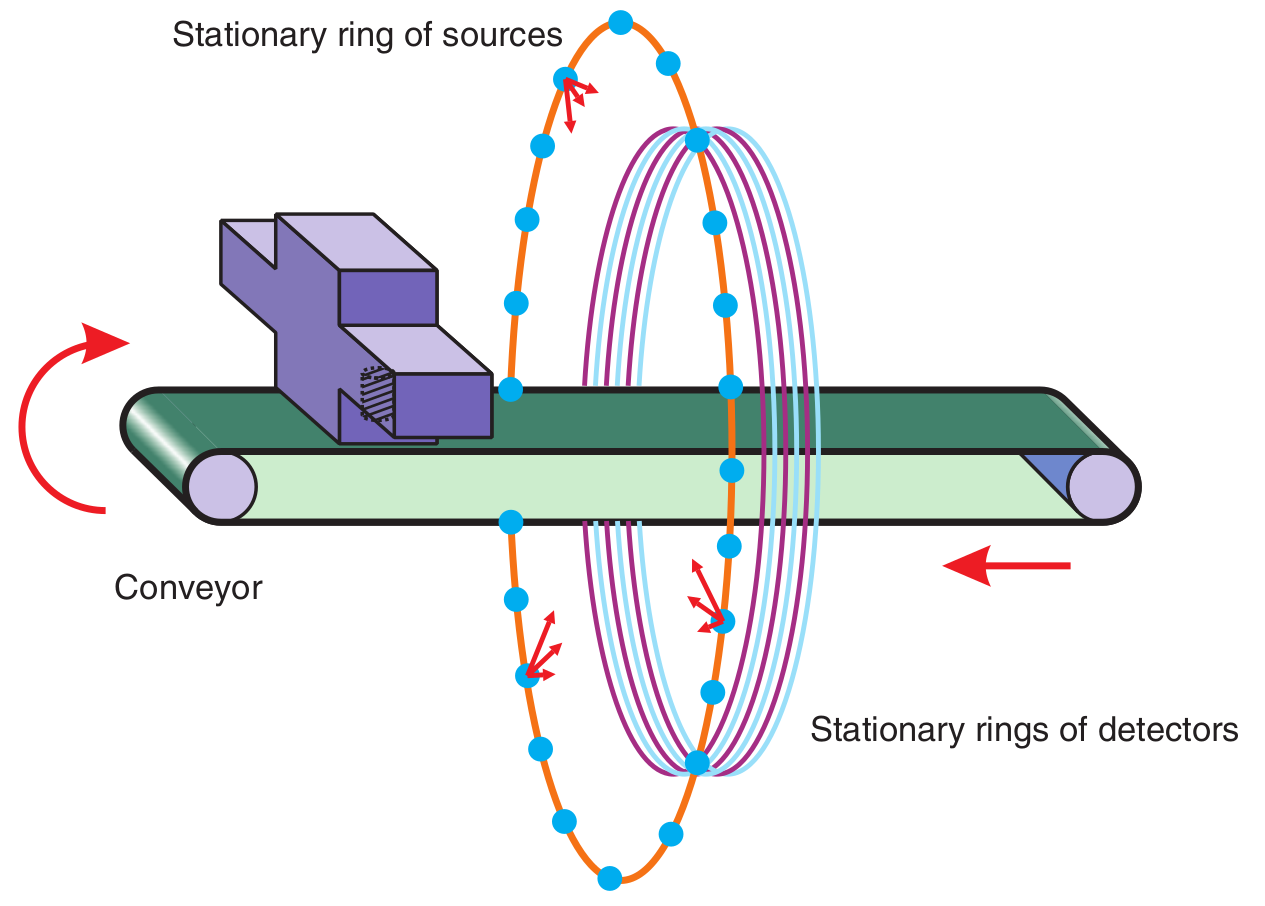
\includegraphics[width=0.7\textwidth]{../figures/literatureReview/literature_conveyor.png}
  \caption{XCT can be done on a conveyor belt surrounded by x-ray source and detector pairs. Reprinted from \cite{warnett2016towards} under the CC BY 3.0 license.}
  \label{fig:literature_conveyor}
\end{figure}

Instead of reconstructing the object, the analysis can be done on the projections itself, or in projection space, by comparing it to a simulated projection produced by a software called \emph{aRTist} \citep{bellon2007artist, jaenisch2008artist, bellon2012radiographic}. It can simulate projections of the object given the specifications of the CT apparatus, such as the x-ray source and the x-ray detector, and the CAD of the object \citep{bellon2011simulation, deresch2012simulating}.

An algorithm was developed to adjust the parameters of the simulation as well as aligning it so that it fits with the x-ray acquisition \citep{brierley2018optimized}. However, it is very complicated as it is optimising over a very large dimensional space \citep{brierley2018optimized}. It was demonstrated that detection of defects is possible in projection space by comparing two simulated projections with each other, one with defects and the other without \citep{brierley2018optimized}. Another method is to use machine learning methods to classify defects from a projection \citep{rale2009comparison}.

It is however inevitable that accuracy is lost from the transition from reconstruction space to projection space, for example, in the diagnostic of pneumonia, a CT scan has superior performance compared to a chest radiograph \citep{hayden2009chest}.